\documentclass[a4paper]{book}

% hiperlinkovi - url i href
\usepackage{url}

% dodatne matematicke oznake
\usepackage{amssymb}
\usepackage{amsmath}
\usepackage{amsthm}

% jezicki paketi
\usepackage[serbian]{babel} % podrska za srpski jezik
\usepackage[utf8]{inputenc} % podrska za utf8 kodiranje

% izgled strane i boje
\usepackage[hmarginratio=1:1, bottom = 1.5in]{geometry}
\PassOptionsToPackage{svgnames}{xcolor}

% paketi za crtanje grafike
\usepackage{tikz}
\usetikzlibrary{intersections, calc, backgrounds, shapes.misc, arrows, petri, topaths, decorations.markings, automata, positioning}

% bojenje hiperlinkova
\usepackage[colorlinks=true, linkcolor=red!80, citecolor=green, urlcolor=blue]{hyperref}

% za podesavanje elemenata na strani
\usepackage{adjustbox}

% napredne figure i tabele
\usepackage{caption}
\usepackage{float}

% podesavanje hedera i futera
\usepackage{fancyhdr}	
\pagestyle{fancy}
\fancyhead{} 
\fancyhead[RO,RE]{\thepage}
\fancyhead[LO,LE]{\slshape \leftmark}
\fancyfoot{} 
\fancyfoot[C]{ }

% za napredne kodove - koristi se okruzenje "lstlisting"
\usepackage{listings}
% na pocetku svakog POGLAVLJA potrebno je pozvati narednu komandu
\newcommand{\setbookcodestyle}{
	\lstset{
		basicstyle=\ttfamily,
		columns=fullflexible,
		keepspaces=true,
		showstringspaces=false,
		escapechar=\%,
		tabsize=4,
		breaklines=true,
		postbreak=\mbox{\textcolor{red}{$\hookrightarrow$}\space},
		frame=None,
		keywordstyle=\color{black},
	   	commentstyle=\color{black},
	   	identifierstyle=\color{black},
	   	stringstyle=\color{black}
	}
}
% na pocetku svake sekcije koja sadrzi KODOVE SA VEZBI potrebno je pozvati narednu komandu
\newcommand{\setexamplecodestyle}{
	\lstset{
		basicstyle=\ttfamily,
		columns=fullflexible,
		keepspaces=true,
		showstringspaces=false,
		escapechar=\%,
		tabsize=4,
		language=Python,
		breaklines=true,
		postbreak=\mbox{\textcolor{red}{$\hookrightarrow$}\space},
		frame=L,
	   	keywordstyle=\bfseries\color{green!40!black},
	   	commentstyle=\itshape\color{purple!40!black},
	   	identifierstyle=\color{blue},
	   	stringstyle=\color{orange}
	}
}

% dodatna okruzenja
\newtheorem{definicija}{Definicija}[chapter]
\newtheorem{teorema}[definicija]{Teorema}
\newtheorem{lema}[definicija]{Lema}
\newtheorem{primer}[definicija]{Primer}
\newtheorem{zadatak}[definicija]{Zadatak}
\newtheorem*{dokaz}{Dokaz}


\usepackage{mdframed}
\newtheorem{Problem}{Problem}
\newenvironment{problem}
{\begin{mdframed}\begin{Problem}}
		{\end{Problem}\end{mdframed}}

% dodatne komande
\newcommand{\blankpage}{\newpage\hbox{}\thispagestyle{empty}\newpage}
\renewcommand\qedsymbol{\hspace*{\stretch{1}} $\blacksquare$}
\usepackage{tcolorbox}
\begin{document}

\begin{titlepage}
	\vspace*{0.4\textheight}
	
	\begin{center}
		{\Huge \textsc{Bioinformatika}}
	\end{center}
	
	\vfill
	
	\begin{center}
		{\Large \today.}
	\end{center}
\end{titlepage}

\blankpage

\frontmatter
\tableofcontents
\blankpage

\chapter*{Predgovor}
Tekst se sastoji od proširenih beleški sa predavanja na osnovu knjige Pavel A. Pevzner, Phillip Compeau: Bioinformatics Algorithms: An Active Learning Approach. \\Tekst su sastavili studenti sa kursa održanog u školskoj 2017/2018 godini: 
\begin{itemize}
	\item Una Stanković 1095/2016
	\item Marina Nikolić 1055/2017
	\item Strahinja Milojević 1049/2017
	\item Anja Bukurov 1082/2016
	\item Nikola Ajzenhamer 1083/2016
	\item Vojisalv Stanković 1080/2016
\end{itemize}


\blankpage

\mainmatter
\chapter{Gde u genomu počinje replikacija genoma?}
\section{Uvod}
\label{sec:uvod}

Na samom početku, želimo da definišemo pojam bioinformatike i da pokušamo da shvatimo koji je njen osnovni cilj. Da bismo to postigli, pogledajmo tri definicije, iz različitih izvora:

\begin{itemize}
  \item $"$Bioinformatika je nauka koja se bavi prikupljanjem i analizom kompleksnih bioloških podataka poput genetskih kodova.$"$ - Oksfordski rečnik (engl. \textit{Oxford Dictionary})
  \item $"$Bioinformatika predstavlja prikupljanje, klasifikaciju, čuvanje i analizu biohemijskih i bioloških informacija korišćenjem računara, a posebno se primenjuje u molekularnoj genetici i genomici.$"$ - Rečnik Meriam-Vebster (engl. \textit{Merriam-Webster Dictionary}) 
 \item $"$Bioinformatika je interdisciplinarno polje koje radi na razvoju metoda i softverskih alata za razumevanje bioloških podataka.$"$ - Vikipedija (engl. \textit{Wikipedia}) 
\end{itemize}

Na osnovu ove tri definicije možemo zaključiti da:\\
\textit{Bioinformatika predstavlja primenu računarskih tehnologija u istraživanjima u oblasti biologije i srodnih nauka.}\\\\
Bioinformatika ima široku primenu i njene primene rastu zajedno sa razvojem discipline. Kao što možemo videti na slici ispod, primena bioinformatike se može sagledati kroz personalizovanu medicinu. Naime, na osnovu prikupljene veće količine podataka i njihove analize, uz pomoć različitih računarskih metoda, na primer metoda veštačke inteligencije, možemo doći do informacija potrebnih da na najbolji način lečimo pacijenta ili mu odredimo terapiju koja će mu na najbolji, najbrži i najbezbolniji način pomoći da prevaziđe određene zdravstvene probleme.  \\

\begin{figure}[h]
\caption{Primena bioinformatike}
\centering
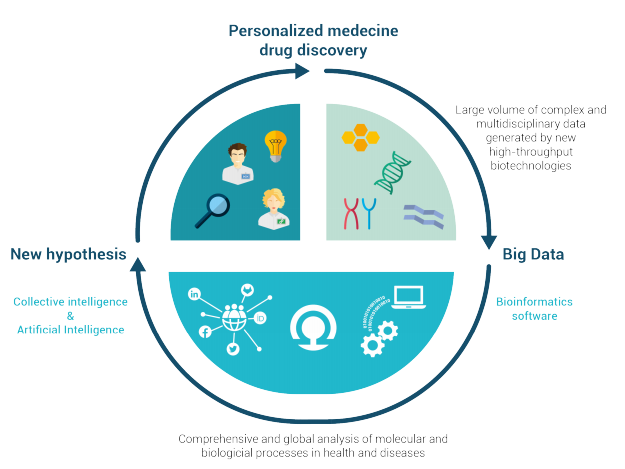
\includegraphics[width=0.7\textwidth]{poglavlja/1/slike/Primena.png}
\end{figure} 

Bioinformatika je spoj više različitih disciplina, kao što su:
\begin{itemize}
	\item Statistika
	\item Istraživanje podataka	
	\item Računarstvo
	\item Računarska biologija
	\item Biologija
	\item Biostatistika
\end{itemize}
Prikaz preklapanja ovih disciplina možemo videti na slici 1.2.
\begin{figure}[h]
\caption{Preklapanjem različitih disciplina dobijamo bioinformatiku.}
\centering
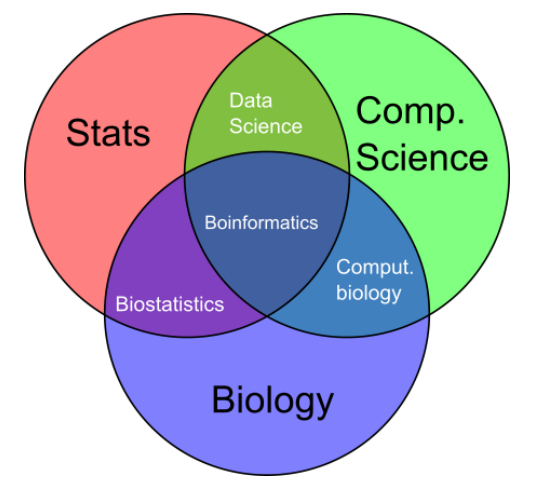
\includegraphics[width=0.7\textwidth]{poglavlja/1/slike/Multidisciplinarnost.png}
\end{figure}  

\newpage

\section{Replikacija genoma}
\label{sec:replikacija}

\subsection{DNK}

Dezoksiribonukleinska kiselina (akronimi DNK ili DNA, od engl. \textit{ deoxyribonucleic acid}), nukleinska kiselina koja sadrži uputstva za razvoj i pravilno funkcionisanje svih živih organizama. Zajedno sa RNK i proteinima, DNK je jedan od tri glavna tipa makromolekula koji su esencijalni za sve poznate forme života. \\\\
Sva živa bića svoj genetički materijal nose u obliku DNK, sa izuzetkom nekih virusa koji imaju ribonukleinsku kiselinu (RNK). DNK ima veoma važnu ulogu ne samo u prenosu genetičkih informacija sa jedne na drugu generaciju, već sadrži i uputstva za građenje neophodnih ćelijskih organela, proteina i RNK molekula. DNK segment koji sadrži ova važna uputstva se naziva gen.\\\\

DNK se sastoji iz dva polimerna lanca koji imaju antiparalelnu orijentaciju, i svaki od njih je sastavljen od azotnih baza:
\begin{itemize}
	\item adenin (A)
	\item timin (T)
	\item guanin (G)
	\item citozin (C)
\end{itemize}

\begin{figure}[h]
\caption{Prikaz DNK, slika preuzeta sa https://ghr.nlm.nih.gov/primer/basics/dna}
\centering
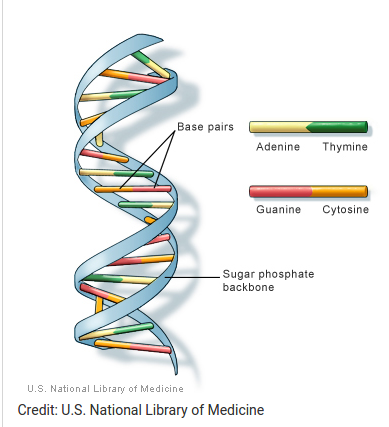
\includegraphics[width=0.5\textwidth]{poglavlja/1/slike/DNK.png}
\end{figure} 

Lanci DNK su međusobno spojeni i to tako da se veze uspostavljaju isključivo između adenina i citozina ili između guanina i timina. Na osnovu toga, ako nam je poznat sastav jednog lanca, lako možemo zakljuciti i sastav drugog lanca, zbog čega se kaže da su DNK lanci \textbf{međusobno komplementarni}.\\\\
Da bismo lakše manipulisali sa informacijama koje DNK nosi i približili sadržaj računarskoj struci, DNK ćemo posmatrati kao nisku nad azbukom \textit{A,C,G,T}.

\subsection{Replikacija genoma u ćeliji}
Replikacija genoma je jedan od najvažnijih zadataka ćelije. Pre nego što se podeli, ćelija mora da najpre replicira svoj genom, tako da svaka od ćerki ćelija dobije svoju kopiju. \\\\
Dzejms Votson (engl. \textit{James Watson}) i Fransis Krik (engl. \textit{Fransis Crick}) su 1953. godine napisali rad u kome su primetili da postoji mehanizam za kopiranje genetskog materijala. Oni su uočili da se lanci roditeljskog DNK molekula odvijaju tokom replikacije i da se, potom, svaki lanac ponaša kao uzorak za sintezu novog lanca (na osnovu toga što se uvek spajaju iste aminokiseline A-C i G-T, rekreiranje lanca je moguće). Kao rezultat ovakvog ponašanja, proces replikacije počinje parom komplementarnih lanca i završava se sa dva para komplementarnih lanaca, kao što se može videti na slici ispod.\\\\

\begin{figure}[h]
\caption{Prikaz replikacije}
\centering
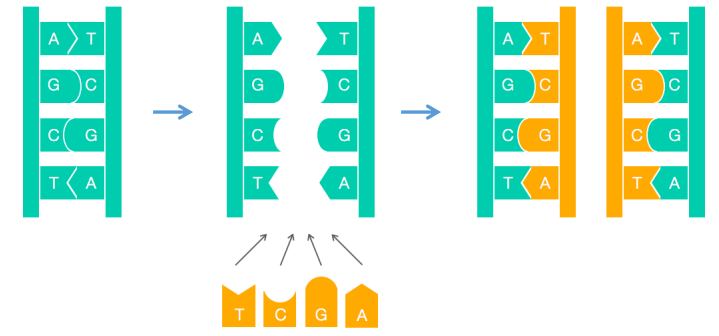
\includegraphics[width=1\textwidth]{poglavlja/1/slike/Replikacija.png}
\end{figure} 

Replikacija počinje u regionu genoma koji se naziva \textbf{početni region replikacije} (skraćeno \textit{oriC}), izvode je enzimi koje se nazivaju DNK polimeraze, koje predstavljaju mašine za kopiranje na molekularnom nivou.\\\\
Nalaženje početnog regiona replikacije predstavlja veoma važan problem, ne samo za razumevanje funkcionisanja kako se ćelije repliciraju, već je koristan i u raznim biomedicinskim problemima. Na primer, neki metodi genskih terapija uključuju genetski izmenjene mini genome, koji se zovu virusni vektori, zbog svoje sposobnosti da prodru kroz ćelijski zid (poput pravih virusa). Virusni vektori u sebi nose veštačke gene koji unapredjuju postojeći genom. Genska terapija je prvi put uspešno izvršena 1990. godine na devojčici koja je bila toliko otporna na infekcije da je bila primorana da živi isključivo u sterilnom okruženju.\\\\
Osnovna ideja genske terapije je da se pacijent, koji pati od nedostatka nekog bitnog gena, zarazi viralnim vektorom koji sadrži veštački gen koji enkodira terapeutski protein. Jednom kad je unutar ćelije, vektor se replicira, što dovodi do lečenja bolesti pacijenta. Da bi moglo da dodje do ovoga, biolozima je neophodno da znaju gde je \textit{oriC}.

\subsubsection{Kako ćelija prepoznaje \textit{oriC}?}
Pitamo se kako ćelija prepoznaje oriC? Sigurno je da postoji neka niska aminokiselina koja označava oriC, ali kako ga prepoznati?\\\\
Ograničimo se na bakterijski genom, koji se sastoji od jednog kružnog hromozoma. Istraživanje je pokazalo da je region, koji predstavlja oriC kod bakterija,
dug svega nekoliko stotina nukleotida.\\\\

\begin{figure}[h]
\caption{Prikaz početka replikacije kod bakterija}
\centering
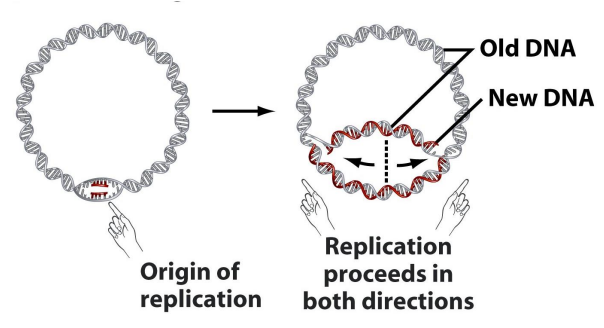
\includegraphics[width=0.7\textwidth]{poglavlja/1/slike/Replikacija_bakterija.png}
\end{figure} 

Poznato je da DNKA utiče na početak replikacije. \textit{DNKA} je protein koji se vezuje na kratki segment unutar oriC, poznatiji kao \textbf{DNKA boks}. Ona predstavlja poruku unutar sekvence DNK koja govori proteinu DNKA da se veže baš tu. Postavlja se pitanje kao pronaći taj region bez prethodnog poznavanja izgleda DNKA boks? \\\\

Da bismo bolje razumeli \textit{problem skrivene poruke} uzmimo za primer priču Edgara Alana Poa - $"$Zlatni jelenak$"$ (engl. \textit{$"$The Gold-Bug$"$}).
Naime, u toj priči jedan od likova, Vilijam Legrand (engl. \textit{William Legrand}), treba da dešifruje poruku :\\

\texttt{53++!305))6*;4826)4+.)4+);806*;48!8`6
0))85;]8*:+*8!83(88)5*!;46(;88*96*?;8\\
)*+(;485);5*!2:*+(;4956*2(5*4)8`8*;40
69285);)6!8)4++;1(+9;48081;8:8+1;48!8
5;4)\\485!528806*81(+9;48;(88;4(+?34;48
)4+;161;:188;+?;}\\\\
On uočava da se $"$;48$"$ pojavljuje veoma često, i da verovatno predstavlja $"$THE$"$, najčešću reč u engleskom jeziku. Znajući to, zamenjuje karaktere odgovarajućim slovima i postepeno dešifruje celu poruku.\\\\
\texttt{53++!305))6*THE26)H+.)H+)806*THE
!E`60))E5;]E*:+*E!E3(EE)5*!TH6(T
EE*96*?;E)*+\\(THE5)T5*!2:*+(TH956
*2(5*H)E`E*TH0692E5)T)6!E)H++T1(
+9THE0E1TE:E+1\\THE!E5T4)HE5!52880
6*E1(+9THET(EETH(+?34THE)H+T161T
:1EET+?T}\\\\
Želeli bismo da ovaj princip primenimo na naš problem nalaska \textit{oriC}-a. Ideja je da uvidimo da li postoje reči koje se neuobičajeno često pojavljuju. Uvedimo termin k-gram da označimo string dužine $k$ i COUNT(Text, Pattern) da označimo broj puta kojih se k-gram $Pattern$ pojavio u tekstu $Text$. Osnovna ideja je da pomeramo prozor, iste dužine kao k-gram $Pattern$, niz tekst, usput proveravajući da li se pojavljuje $Pattern$ u nekome od njih. 

\begin{lstlisting}
PATTERNCOUNT(Text, Pattern)
	count = 0
	for i = 0 to |Text| - |Pattern|
		if Text(i,|Pattern|) = Pattern
			count = count + 1 
	return count
\end{lstlisting}
	
Za neki $Pattern$ kažemo da je on \textit{najčešći k-gram} u tekstu $Text$, ako je njegov $COUNT$ najveći među svim k-gramima. Na primer, \textbf{ACTAT} je najčešći 5-gram u tekstu $Text$ = ACA\textbf{ACTAT}GCA\textbf{ACTAT}CGGGACA\textbf{ACTAT}CCT, a \textbf{ATA} je najčešći 3-gram u $Text$ = CG\textbf{ATATA}TCC\textbf{ATA}G.\\\\
Sada, problem pronalaska čestih reči možemo posmatrati kao računarski problem:\\
\begin{tcolorbox}
\textbf{Problem čestih reči:} Pronaći najčešće k-grame u niski karaktera.\\
\textit{Ulaz:} Niska Text i ceo broj k.\\
\textit{Izlaz:} Svi najčešći k-grami u niski Text. \\\\
\end{tcolorbox}
Osnovni algoritam za pronalazak čestih k-grama u stringu $Text$ proverava sve k-grame koji se pojavljuju u tom stringu (takvih k-grama ima $|Text|-k+1$) i potom izračunava koliko puta se svaki k-gram pojavljuje. Da bismo implementirali ovaj algoritam, moramo da izgenerišemo niz $COUNT$, gde je $COUNT(i) = COUNT(Text, Pattern)$ za $Pattern = Text(i,k)$.\\

\begin{lstlisting}
FrequentWords(Text, k)
	FrequentPatterns <- an empty set
	for i = 0 to |Text| - k
		Pattern <- the k-mer Text(i,k)
		COUNT(i) <- PatternCount(Text, Pattern)
	maxCount <- max value in array COUNT
	for i = 0 to |Text| - k
		if COUNT(i) = maxCount
			add Text(i,k) to FrequentPatterns
	remove duplicates from FrequentPatterns
	return FrequentPatterns
\end{lstlisting}

Pitamo se, sada, kolika je složenost ovakvog pristupa?\\
Ovaj algoritam, iako uspešno nalazi ono što se od njega traži, nije najefikasniji. S obzirom na to da svaki k-gram zahteva $|Text|-k+1$ provera, svaki od njih zahteva i do $k$ poređenja, pa je broj koraka izvršavanja funkcije $PatternCount(Text, Pattern)$ zapravo $(|Text|-k+1)*k$. Osim toga, $FrequentWords$ mora pozvati $PatternCount$ $|Text|-k+1$ puta (po jednom za svaki k-gram teksta), tako da je ukupan broj koraka \textit{$(|Text|-k+1)*(|Text|-k+1)*k$}.\\Iz navedenog, možemo zaključiti da je ukupna cena izvršavanja algoritma $FrequentWords$ \textbf{$O(|Text|^2*k)$}.

\subsubsection{Primer: Pronalazak čestih reči kod bakterije \textit{Vibrio cholerae}} 

Posmatrajmo, najpre, tablicu najčešćih k-grama u \textit{oriC} regionu bakterije \textit{Vibrio cholerae}. Da li nam se čini da se neki k-grami pojavljuju neuobičajeno često?\\ 

\begin{figure}[h]
\caption{Tablica najčešćih k-grama u \textit{oriC} regionu bakterije Vibrio cholerae}
\centering
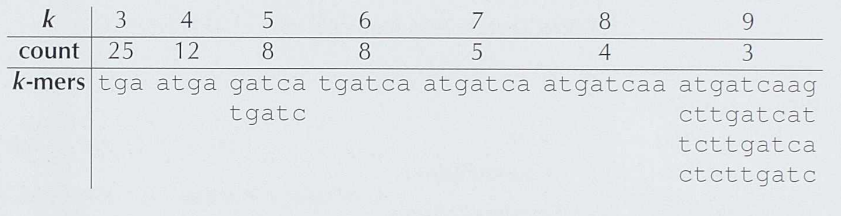
\includegraphics[width=1\textwidth]{poglavlja/1/slike/Tablica_VC.png}
\end{figure} 

Na primer, 9-gram \textbf{ATGATCAAG} se pojavljuje tri puta u \textit{oriC} regionu, da li nas to iznenađuje?\\

\begin{figure}[h]
\caption{Prikaz 9-grama ATGATCAAG i njegovog komplementa u \textit{oriC} regionu Vibrio cholerae}
\centering
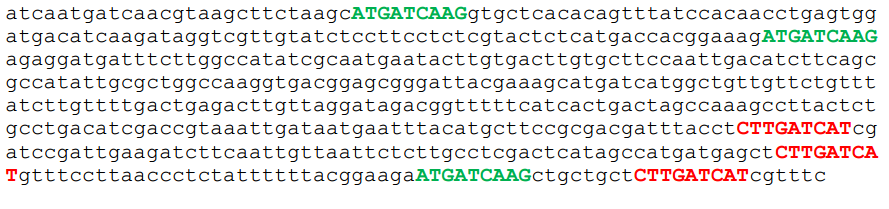
\includegraphics[width=1\textwidth]{poglavlja/1/slike/9_VC.png}
\end{figure} 

Označili smo najčešće 9-grame, umesto nekih drugih k-grama, jer je eksperimentima pokazano da su DNKA boksovi kod bakterija dugi 9 nukleotida. Verovatnoća da postoji 9-gram koji se pojavljuje 3 ili više puta u proizvoljno generisanom DNK stringu dužine 500 je $1/1300$. Uočimo da postoje četiri različita 9-grama koji se ponavljaju tri ili više puta u ovom regionu, to su: ATGATCAAG, CTTGATCAT, TCTTGATCA i CTCTTGATC.\\\\

Mala verovatnoća da se neki 9-gram toliko puta pojavi u \textit{oriC}-u kolere, govori nam da neki od četiri 9-grama koje smo pronašli može biti potencijalni DNKA boks, koji započinje replikaciju. Ali, koji?\\\\

Podsetimo se da nukleotidi A i T, kao i C i G, su komplementarni. Ako imamo jednu stranu lanca DNK i neke slobodne nukleotide, možemo lako zamisliti sintezu komplementarnog lanca, kao što se vidi na slici ispod. 

\begin{figure}[h]
\caption{Komplementarni lanci se $"$kreću$"$ u suprotnim smerovima.}
\centering
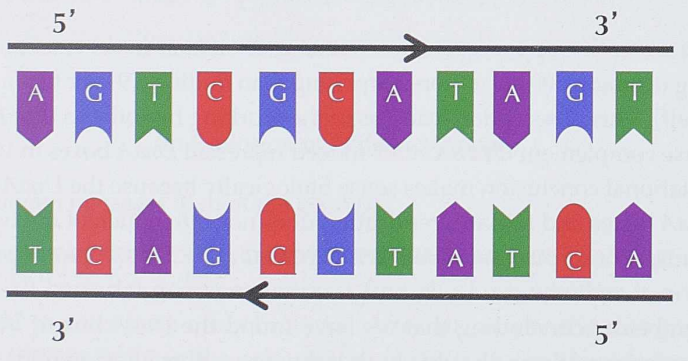
\includegraphics[width=1\textwidth]{poglavlja/1/slike/Komplementarni.png}
\end{figure} 

Posmatrajmo ponovo sliku 1.7. Na njoj možemo uočiti 6 pojavljivanja niski ATGATCAAG i CTTGATCAT, koji su zapravo komplementarni. Naći 9-gram koji se pojavljuje 6 puta u DNK nisci dužine 500 nukleotida, je još više iznenadjujuće, nego pronaći 9-gram koji se pojavljuje tri puta. Ovo posmatranje nas dovodi do toga da je ATGATCAAG (zajedno sa svojim komplementom) zaista DNKA boks Vibrio cholerae. Ovaj zaključak ima i smisla biološki, jer DNKA proteinu, koji se vezuje i započinje replikaciju, nije bitno za koji od dva lanca se vezuje.\\\\

\subsubsection{Primer: Pronalazak čestih reči kod bakterije \textit{Thermotoga petrophila}} 

Nakon što smo pronašli skrivenu poruku za Vibrio cholerae, ne bi trebalo da odmah zaključimo da je ta poruka ista kod svih bakterija. Najpre bi trebalo da proverimo da li se ona nalazi u \textit{oriC} regionu drugih bakterija, možda različite bakterije, imaju drugačije DNKA boksove. Uzmimo, za primer, \textit{oriC} region bakterije Thermotoga petrophila. Ona predstavlja bakteriju koja obitava u izrazito toplim regionima, na primer u vodi ispod rezervi nafte, gde temperature prelaze 80 stepeni Celzijusa. Pogledajmo kako izgleda \textit{oriC} region ove bakterije.

\begin{figure}[h]
\caption{Prikaz \textit{oriC} regiona Thermotoga petrophila}
\centering
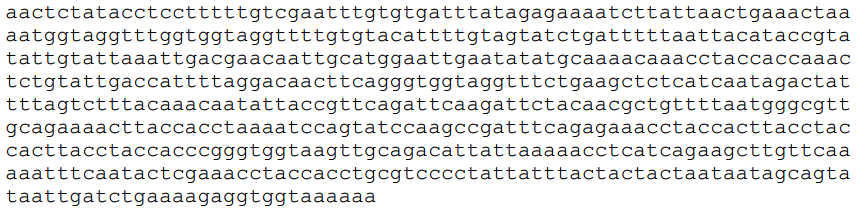
\includegraphics[width=1\textwidth]{poglavlja/1/slike/OriC_TP.png}
\end{figure} 

Možemo lako uočiti da se u ovom regionu nigde ne javljaju niske ATGATCAAG ili CTTGATCAT, iz čega zaključujemo da različite bakterije mogu koristiti različite DNKA boksove, kako bi pružile skrivenu poruku DNKA proteinu. Odnosno, za različite genome imamo različite DNKA boksove.

Najčešće reči u ovom \textit{oriC} su:
\begin{itemize}
	\item AACCTACCA, 
	\item ACCTACCAC,
	\item GGTAGGTTT,
	\item TGGTAGGTT,
	\item AAACCTACC,
	\item CCTACCACC
\end{itemize}

Pomoću alata koji se zove Ori-Finder, nalazimo CCTACCACC i njegov komplement GGTGGTAGG kao potencijalne DNKA boksove naše bakterije. Ove dve niske se pojavljuju ukupno 5 puta.

\begin{figure}[h]
\caption{Prikaz CCTACCACC i njenog komplementa u \textit{oriC} regionu Thermotoga petrophila}
\centering
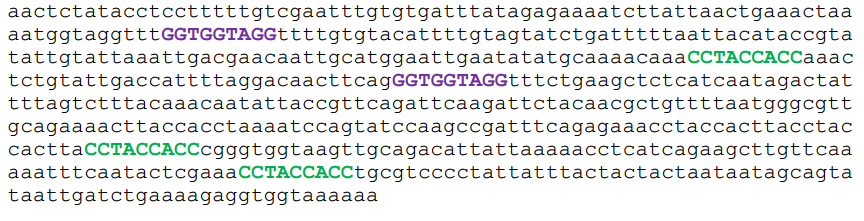
\includegraphics[width=1\textwidth]{poglavlja/1/slike/TP.png}
\end{figure} 
Naučili smo da pronađemo skrivene poruke ako je \textit{oriC}
dat, ali ne znamo da pronađemo \textit{oriC} u genomu.

\subsection{Pronalaženje početnog regiona replikacije}

Zamislimo da pokušavamo da nađemo \textit{oriC} u novom sekvenciranom genomu bakterije. Ako bismo tražili niske poput ATGATCAAG/CTTGATCAT ili CCTACCACC/GGTGGTAGG to nam verovatno ne bi bilo puno od pomoći, jer novi genom može koristiti potpuno drugačiju skrivenu poruku. Posmatrajmo, zato, drugačiji problem: umesto da tražimo grupe određenog k-grama, pokušajmo da nađemo svaki k-gram koji formira grupu u genomu. Nadajmo se da će nam lokacije ovih grupa u genomu pomoći da odredimo lokaciju \textit{oriC}-a.\\Ideja je da pomeramo prozor fiksirane dužine L kroz genom, tražeći region u kome se k-gram pojavljuje više puta uzastopno. Za L ćemo uzeti vrednost 500, koja predstavlja najčešću dužinu \textit{oriC}-a kod bakterija. \\\\
Definisali smo k-gram kao \textit{grupu}, ako se pojavljuje više puta unutar kratkog intervala u genomu. Formalno, k-gram Pattern formira (L, t) grupu unutar niske Genome ako postoji interval genoma, dužine L, u kome se k-gram pojavljuje barem t puta. \\\\
\begin{tcolorbox}
\textbf{Problem pronalaženja grupa.} Naći k-grame koji
formiraju grupe unutar niske karaktera.\\
Ulaz. Niska Genome i celi brojevi k (dužina
podniske), L (dužina prozora) i t (broj podniski u
grupi).\\
Izlaz. Svi k-grami koji formiraju (L, t)-grupe u
niski Genome.
\end{tcolorbox}

U genomu bakterije E.coli postoji 1904 različitih 9-
grama koji formiraju (500,3)-grupe. Koji od njih
ukazuje na početni region replikacije?

\subsubsection{Iskrivljeni dijagrami}

S obzirom na to da imamo veliku količinu statističkih podataka, pitamo se kako ih možemo upotrebiti da bismo došli do lokacije \textit{oriC}-a? U tome nam mogu pomoći \textbf{iskrivljeni dijagrami}(engl. \textit{skew diagram}). Osnovna ideja je da prođemo kroz genom i da računamo razliku između količine guanina(G) i citozina(C). Ako ova razlika raste, onda možemo pretpostaviti da se krećemo niz polulanac koji ide na desno (u nastavku samo polulanac, smer $5'-> 3'$), a ako razlika počne da se smanjuje, onda pretpostavljamo da smo na obrnutom polulancu ($3' -> 5'$). Zbog procesa koji se naziva deaminacija (gubljenje aminokiselina), svaki polulanac ima manjak citozina u poređenju sa guaninom, a svaki obrnuti polulanac ima manjak guanina u odnosu na citozin. 

\begin{figure}[h]
\caption{Prikaz kretanja.}
\centering
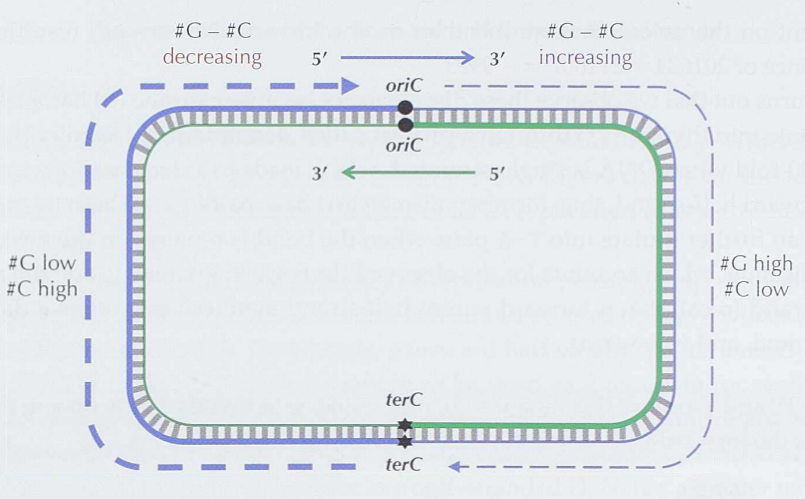
\includegraphics[width=1\textwidth]{poglavlja/1/slike/Polulanci_CG.png}
\end{figure} 

\begin{figure}[h]
\caption{Iskrivljeni dijagram genoma Genome = CATGGGCATCGGCCATACGCC.}
\centering
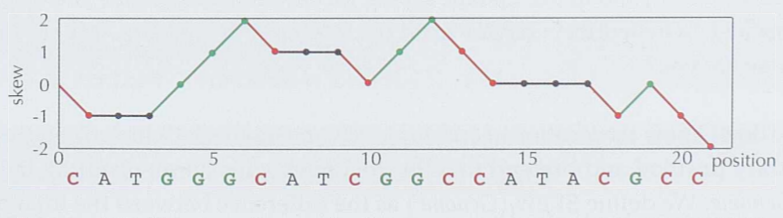
\includegraphics[width=1\textwidth]{poglavlja/1/slike/skew.png}
\end{figure} 

Posmatrajmo iskrivljeni dijagram bakterije Ešerihija Koli. Lako uočavamo minimalnu vrednost skew dijagrama.

\begin{figure}[h]
\caption{Iskrivljeni dijagram Ešerihije koli.}
\centering
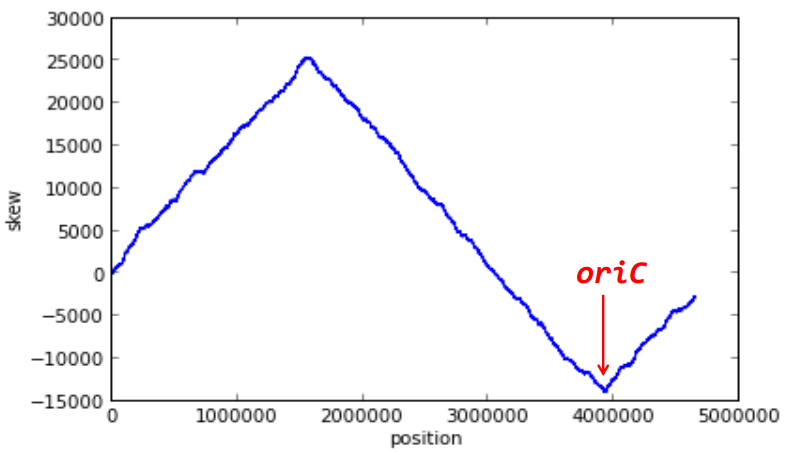
\includegraphics[width=1\textwidth]{poglavlja/1/slike/Ecoli_oriC.png}
\end{figure} 

Minimalna vrednost iz iskrivljenog dijagrama ukazuje baš na ovaj region:

\begin{figure}[H]
\caption{Region na koji pokazuje minimalna vrednost iskrivljenog dijagrama Ešerihije koli.}
\centering
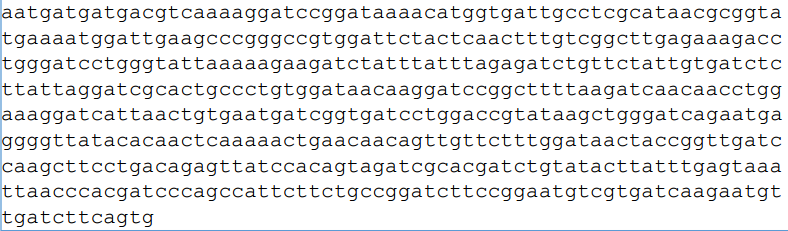
\includegraphics[width=1\textwidth]{poglavlja/1/slike/ecoli_region.png}
\end{figure} 

Uočimo da u ovom regionu nema čestih 9-grama (koji se pojavljuju 3 ili više puta). Iz toga zaključujemo da, iako smo uspeli da nađemo \textit{oriC} bakterije Ešerihija koli, nismo uspeli da nađemo DNKA boksove. Međutim, pre nego što odustanemo od potrage, osmotrimo još jednom \textit{oriC} Vibrio colerae, kako bismo pokušali da nađemo način da izmenimo naš algoritam i uspemo da lociramo DNKA boksove u Ešerihiji koli. Veoma brzo, može se uvideti da osim tri pojavljivanja ATGATCAAG i tri pojavljivanja CTTGATCAT, \textit{oriC} Vibrio cholerae sadrži i dodatna pojavljivanja ATGATCAAC i CATGATCAT koji se razlikuju samo u jednom nukleotidu od gornjih niski. Ovo još više povećava šanse da smo naišli na prave DNKA boksove, a ima i biološkog smisla. Naime, DNKA se može vezati i za nesavršene DNKA boksove, one koji se razlikuju u nekoliko nukleotida.\\\\


\begin{figure}[H]
\caption{Prikaz pojavljivanja nesavršenih niski nukleotida.}
\centering
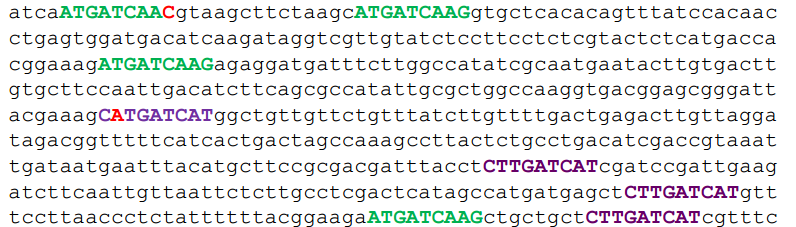
\includegraphics[width=1\textwidth]{poglavlja/1/slike/nesavrseni1.png}
\end{figure} 

Cilj nam je da sada izmenimo algoritam čestih reči (FrequentWords) tako da možemo da pronađemo DNKA boksove koji su predstavljeni čestim k-gramima, sa mogućim izmenama na pojedinim nukleotidima. Ovaj problem nazvaćemo problem čestih reči sa propustima.\\\\
\begin{tcolorbox}
\textbf{Problem čestih reči sa propustima.} Pronaći najčešće k-grame sa
propustima u niski karaktera.\\
Ulaz: Niska Text i celi brojevi k i d.\\
Izlaz: Svi najčešći k-grami sa najviše d propusta u niski Text. \\
\end{tcolorbox}
Pokušajmo, još jednom, sa pronalaskom DNKA boksova kod Ešerihije koli, tako što ćemo naći najčešće 9-grame sa propustima i komplementima u regionu \textit{oriC} koji nam je predložen minimalnom vrednošću iskrivljenog dijagrama. Pokušaćemo sa malim prozorom koji ili počinje ili se završava ili je centriran na poziciji najmanje iskrivljenosti. Ovakvim izvođenjem pronalazimo TTATCCACA/TGTGGATAA kao najčešći 9-gram. Međutim, ovo nije jedini 9-gram. Za ostale 9-grame još uvek ne znamo čemu služe, ali znamo da nose skrivene informacije, da se grupišu unutar genoma i da većina njih nema veze sa replikacijom. 

\begin{figure}[H]
\caption{Prikaz pronađenih niski sa propustima i komplementima u \textit{oriC} regionu Ešerihije koli.}
\centering
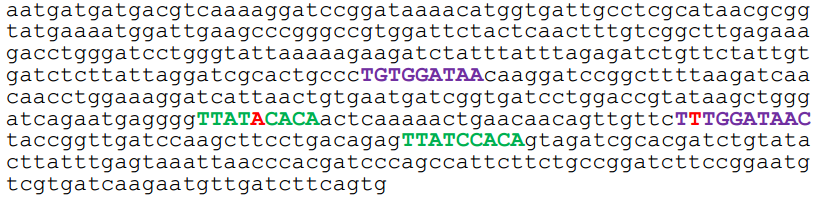
\includegraphics[width=1\textwidth]{poglavlja/1/slike/ecoli_poslednji.png}
\end{figure} 

\newpage

\section{Zadaci sa vežbi}
U nastavku će biti predstavljeni zadaci sa vežbi na kursu rađeni u programskom jeziku Python.

\subsection{FrequentWords}

\lstinputlisting[language=Python]{poglavlja/1/kodovi/1.py}

\subsection{Faster FrequentWords}

\lstinputlisting[language=Python]{poglavlja/1/kodovi/3.py}

\subsection{Skew Diagram}

\lstinputlisting[language=Python]{poglavlja/1/kodovi/4.py}

\subsection{FrequentWords With Mismatches}

\lstinputlisting[language=Python]{poglavlja/1/kodovi/5.py}


\chapter{Kako složiti genomsku slagalicu od milion delova?}

\section{Šta je sekvenciranje genoma?}

Sa biološke strane, genom jednog organizma predstavlja njegov genetski materijal. Kod većine organizama, genetski materijal je sadržan u DNK. Kod čoveka, genom sadrži oko tri milijarde nukleotida. Genomi nekih organizama su i 100 puta veći od humanog genoma. 

Sa računarske strane, genom je niska karaktera nad azbukom $\{A, C, G, T\}$.

% nije mi jasan veliki razmak koji se napravi  u tekstu na ovom mestu xD

\subsection{Kratka istorija sekvenciranja genoma}

1977. godine Walter Gilbert i Frederick Sanger razvijaju nezavisne metode sa sekvenciranje DNK, za koje su, 1098. godine, podelili su Nobelovu nagradu.
Njihove metode za sekvenciranje su bile veoma skupe - 3 milijarde dolara za sekvenciranje humanog genoma.
\\
\\
Krajem 2000-tih Sanger metodom je sekvencioniran veliki broj genoma. Visoka cena je bila ograničavajući faktor i za dalji napredak je bila neophodna nova tehnologija sekvencioniranja.
\\
\\
\textbf{NGS} predstavlja metode nove generacije sekvencioniranja. Krajem 2000-tih, na tržištu se pojavljuju nove mašine za sekvenciranje. \textit{Illumina} smanjuje trošak sekvencioniranja humanog gemona sa 3 milijarde na 10 hiljada dolara. Kompanija \textit{Complete Genomics} otvara genomsku fabriku u Silikonskoj dolini koja sekvencionira stotine genoma mesečno.
Pekinški genomski institut (BGI - Beijing Genome Institute) preuzima Complete Genomics 2013. godine i postaje najveći svetski centar za sekvenciranje genoma.
Na slici \ref{slika:cena} prikazano je kako se cena sekvencioniranja menjala godinama.


\begin{figure}[H]
	\centering
	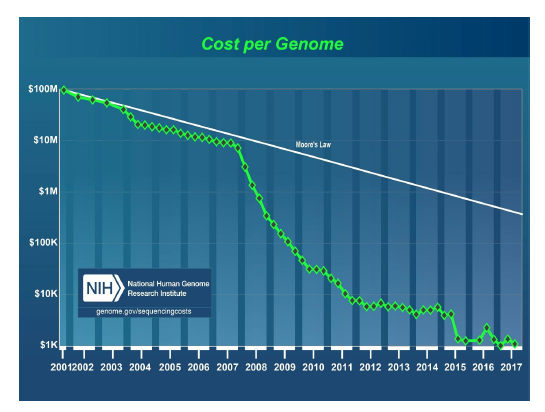
\includegraphics[width=1\textwidth]{poglavlja/3/slike/cena_sekvencioniranja.png}
	\caption{Cena sekvencioniranja kroz istoriju.}
	\label{slika:cena}
\end{figure} 



\subsection{Sekvenciranje ličnih genoma}

Genomi se kod različitih ljudi razlikuju na malom broju pozicija (u proseku sadrže jednu mutaciju na hiljadu nukleotida). Ova razlika je odgovorna za različite visine kod ljudi, da li će imati sklonost ka visokom holesterolu ili ne, za veliki broj genetskih bolesti, itd.
\\
\\
2010: Nicholas Volker je postao prvo ljudsko biće čiji je život spašen zahvaljujući genomskom sekvencioniranju.
Lekari nisu mogli da postave tačnu dijagnozu i morali su da ga podvrgnu velikom broju operacija pokušavajući da je utvrde. Sekvenciranje je otkrilo retku mutaciju na jednom genu (XIAP) koja je bila povezana sa oštećenjem njegovog imunog sistema. Ovo otkriće je navelo lekare na adekvatnu terapiju koja je rešila problem.

\section{Eksplozija u štampariji}

Zamislite da imamo hiljadu kopija istog izdanja novina na jednoj gomili, a ispod njih postavljen je dinamit. Upalimo fitilj i zamislimo da nije sve samo izgorelo već da se raspršilo u milione delića papira. Kako možemo da iskoristimo te deliće da bismo saznali koje su bile vesti iz tog izdanja? Ovaj problem nazvaćemo \textbf{Problem novina} (\ref{slika:eksplozija}). 

\begin{figure}[H]
	\centering
	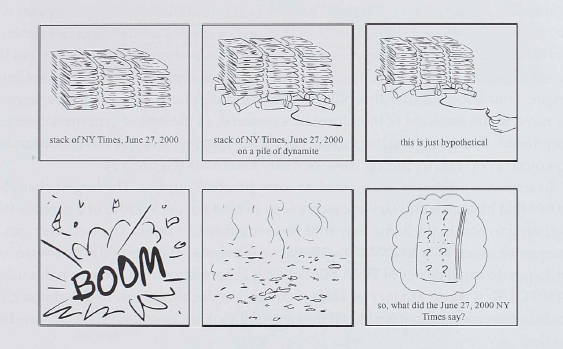
\includegraphics[width=1\textwidth]{poglavlja/3/slike/eksplozija.png}
	\caption{Problem novina poslužiće nam u razumevalju problema slaganja genoma.}
	\label{slika:eksplozija}
\end{figure} 


Problem novina je mnogo teži nego što izgleda. Kako smo imali više kopija istog izdanja, i kako smo izgubili neki deo informacija prilikom eksplozije, ne možemo samo da prilepimo deliće novina kao da su slagalica. Umesto toga, potrebno je da preklopimo delove različitih novina kako bismo rekonstruisali jedan primerak.


\begin{figure}[H]
	\centering
	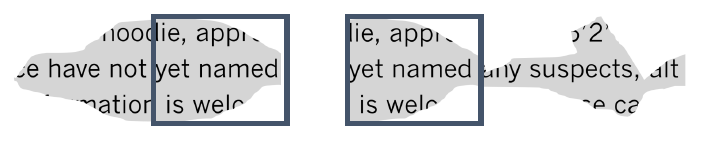
\includegraphics[width=1\textwidth]{poglavlja/3/slike/delici.png}
	\caption{Spajanje delova različitih novina koji se jednim delom preklapaju.}
	\label{slika:delici}
\end{figure} 


Kakve sad to veze ima sa našim problemom? Određivanje redosleda nukleotida u genomu, odnosno sekvenciranje genoma, predstavlja bitan problem u bioinformatici. Dužine genoma variraju: humani genom je dugačak oko 3 milijarde nukleotida, dok je genom jendoćelijskog organizma Amoeba dubia čak 200 puta duži. 


Moderne mašine za sekvenciranje (sekvenceri) ne mogu da pročitaju ceo genom nukleotid po nukleotid od početka do kraja (kao što bismo pročitali knjigu).
Mogu samo da iseckaju genom i generišu njegova kratka očitavanja. Kako to zapravo funkcioniše (\ref{slika:sekvenciranje})? Sekvencer dobija milione kopija istog genoma. Zatim vrši očitavanja čime dobijamo deliće odnosno kratke podniske. Neki delovi odnosno očitavanja biće izgubljena (kao delići novina u eksploziji, dakle gubimo deo informacija). Očitavanja su izmešana i ono što nam sekvencer daje je zapravo kolekcija podniski koje treba spojiti u jednu. Sastavljanje genoma nije isto kao i slaganje slagalice: moramo da koristimo preklapajuća očitavanja da bismo rekonstruisali genom.


\begin{figure}[H]
	\centering
	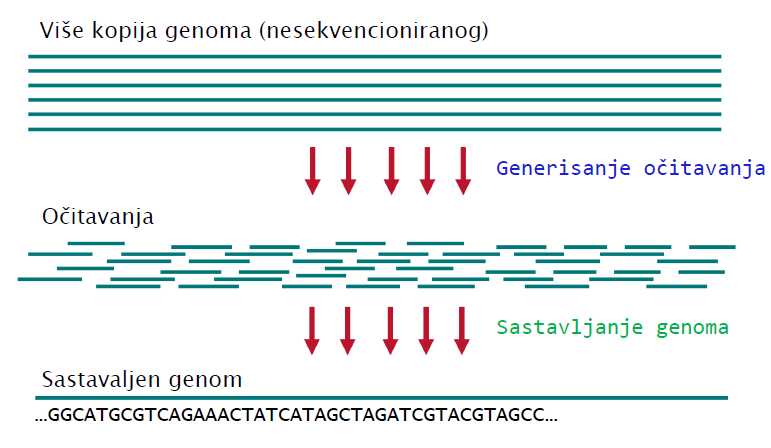
\includegraphics[width=1\textwidth]{poglavlja/3/slike/sekvencioniranje.png}
	\caption{Ilustracija problema.}
	\label{slika:sekvenciranje}
\end{figure} 


\section{Problem sekvenciranja genoma}

\begin{problem}
	[Problem sekvencioniranja genoma] Rekonstruisati genom na osnovu očitavanja.
	\\ Ulaz. Kolekcija niski Reads.
	\\ Izlaz. Niska Genome rekonstruisana na osnovu Reads.
\end{problem}

% ovo dopuniti sa snimka pošto nema ni u knjizi baš
Ovo nije dobro definisan problem. 


\subsection{k-gramski sastav niske}

k-gramski sastav niske $Text$ ($Composition_k(Text)$) predstavlja kolekcija podnsiki dužine $k$ niske $Text$, uključujući duplikate. Na primer:


% ovo sigurno može lepše xD (slajd 32)
\begin{align*}
	Composition_3(TAATGCCATGGGATGTT) =& \\
	TAA AAT ATG TGC GCC CCA CAT ATG TGG GGG GGA GAT ATG TGT GTT =& \\
	AAT ATG ATG ATG CAT CCA GAT GCC GGA GGG GTT TAA TGC TGG TGT
\end{align*}

Sada možemo malo bolje da definišemo problem.

\begin{problem}
	[Problem rekonstrukcije niske] Rekonstruisati nisku na osnovu njenog k-gramskog sastava.
	\\ Ulaz. Kolekcija k-grama.
	\\ Izlaz. Niska Genome takva da je $Composition_k(Genome)$ ekvivalentno kolekciji k-grama
\end{problem}


Naivni pristup ovom problemu bio bi da odaberemo jedan k-gram za početni. Zatim nižemo ostale tako da se sufiks poslednjeg odabranog poklopi sa prefiksom nekog od preostalih k-grama. Pri tome, ako ima više takvih k-grama, biramo jedan, bilo koji, Na ovaj način možemo doći do rešenja, ali je veoma skupo. Pri tome, velika je šansa da ćemo se negde zaglaviti (tj. nijedan od preostalih k-grama neće biti kandidat za nadovezivanje na tekuću nisku) ili zbog izbora početnog k-grama ili zbog izbora nekog od preostalih k-grama kada je postojalo više odgovarajućih. Sledeći primer ilustruje ovaj problem:

Neka nam je dat sledeći 3-gramski sastav: 
$$AAT ATG ATG ATG CAT CCA GAT GCC GGA GGG GTT TAA TGC TGG TGT$$

Treba rekonstruisati nisku koja ima takav sastav. Biramo početni 3-gram, neka to bude na primer $TAA$. Zatim na njega treba nadovezati 3-gram koji počinje njegovim sufiksom dužine 2, odnosno onaj 3-gram koji ima prefiks $AA$. U našem slučaju, postoji jedan takav 3-gram i njega nadovezujemo na tekuću nisku, tako da sada imamo $TAAT$. Zatim biramo 3-gram čiji je prefiks $AT$. Ovog puta imamo 3 kandidata, ali, na našu sreću, sva tri su isti 3-grami, $ATG$. U takvom slučaju nije bitno koji smo odabrali, jer su svi jednaki. Nadovezujemo ga na tekuću nisku i dobijamo $TAATG$. Tražimo 3-grame sa prefiksom $TG$, koji do sad nisu upotrebljeni. Ponovo pronalazimo 3 kandidata. Međutim, u ovom slučaju, svi kandidati predstavljaju različite 3-grame, a to su $TGC$, $TGG$ i $TGT$. Naivni pristup kaže da biramo jedan od njih, i recimo da smo odabrali $TGT$ i dobili nisku $TAATGT$. Sada nam je potrebam 3-gram sa prefiksom $GT$ i tu dolazi do zaglavljivanja! 
Imamo još 3-grama koji nisu iskorišćeni za rekonstrukciju niske, ali nijedan ne možemo da iskoristimo u ovom trenutku! U takvim situacijama treba se vratiti u nazad do koraka u kom je bilo više kandidata.


\section{Rekonstrukcija niske kao problem Hamiltonove putanje}

Videli smo da nam naivni pristup ne odgovara i moramo smisliti bolje rešenje. Mogli bismo da iskoristimo znanja iz teorije grafova za rešavanje ovakvog problema. U tom slučaju, prvi zadatak je da našu nisku predstavimo u vidu grafa.


\subsection{Genom kao putanja}

Vratimo se na prethodni primer. Dat nam je k-gramski sastav niske :
$$Composition_3(TAATGCCATGGGATGTT) =$$
$$ TAA AAT ATG TGC GCC CCA CAT ATG TGG GGG GGA GAT ATG TGT GTT$$

Njega treba predstaviti kao graf. Možemo da napravimo po jedan čvor za svaki od k-grama. Zatim, potrebne su nam grane koje će povezati te čvorove. Dvs čvora su povezana usmerenom granom ako izlazni čvor ima sufiks jednak prefiksu ulaznog čvora te grane, kao što je prikazano na slici \ref{slika:graf1}.

\begin{figure}[H]
	\centering
	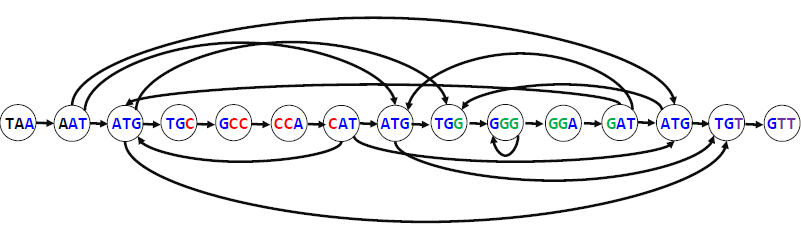
\includegraphics[width=1\textwidth]{poglavlja/3/slike/hamilton.png}
	\caption{Graf koji odgovara k-gramskom sastavu niske $TAATGCCATGGGATGTT$.}
	\label{slika:hamilton}
\end{figure} 

Jasno je da postoji više puteva u ovom grafu. Postavlja se pitanje, da li možemo da pronađemo genomsku putanju u ovom grafu, od svih koje postoje?

Podsetimo se šta je Hamiltonova putanja. Hamiltonova putanja je putanja koja posećuje svaki čvor u grafu tačno jednom. To je upravo ono što nam je potrebno za rešavanje problema. Svaki čvor predstavlja jedan k-gram i porebno nam je da svi k-grami budu uključeni u rekonstruisanu nisku tačno jednom.

\begin{problem}
	[Problem Hamiltonove putanje]
	Naći Hamiltonovu putanju u grafu.
	\\ Ulaz. Graf.
	\\Izlaz. Putanja koja posećuje svaki čvor u grafu tačno jednom.
\end{problem}

Iako deluje kao da smo rešili sve probleme, zapravo smo naišli na još jednu veliku prepreku. Naime, pronalaženje Hamiltonovog puta u grafu je NP-kompletan problem, što znači da ne postoji efikasan algoritam koji to radi.

U tom slučaju, moramo da se vratimo na početak, a to je predstavljanje k-gramskog sastava grafom.


\section{Rekonstrukcija niske kao Ojlerove putanje}


U prethodnoj sekciji k-grame smo predstavili čvorovima u grafu i u njemu tražili Hamiltonov put odnosno put koji obilazi svaki čvor tačno jednom. Videli smo da za taj problem još uvek nije poznat efikasan algoritam pa se sada pitamo kako možemo izmeniti graf tako da ne zahteva traženje Hamiltonove putanje.

Ono što se javlja kao ideja jeste obeležavanje grana umesto čvorova. Dakle, svaka grana biće obeležena jednim k-gramom, podniskama trih k-grama. Izlazni čvor biće obeležen prefiksom k-grama te grane, dok će ulazni čvor biti obeležen sufiksom istog tog k-grama. Na slici \ref{slika:ojler} ilustruje ovaj postupak za nisku $TAATGCCATGGGATGTT$.

\begin{figure}[H]
	\centering
	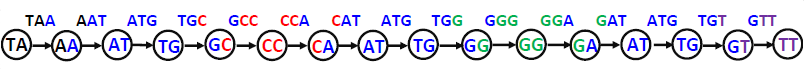
\includegraphics[width=1\textwidth]{poglavlja/3/slike/ojler.png}
	\caption{Graf koji odgovara 3-gramskom sastavu niske $TAATGCCATGGGATGTT$. Grane su obeležene 3-gramima, a čvorovi prefiksima/sufikisima.}
	\label{slika:ojler}
\end{figure} 


Primećujemo da su neki čvorovi obleženi identično (npr. imamo tri čvora sa oznakom $AT$). Sve čvorove koji imaju istu oznaku treba spojiti u jedan, pri čemu zadržavamo sve grane koje su ulazile u taj čvor ili su izlazile iz njega. Ponavljamo postupak dokle god imamo čvorove koji imaju istu oznaku i na kraju dobijamo graf koji nazivamo De Brojnov graf. 

\begin{figure}[H]
	\centering
	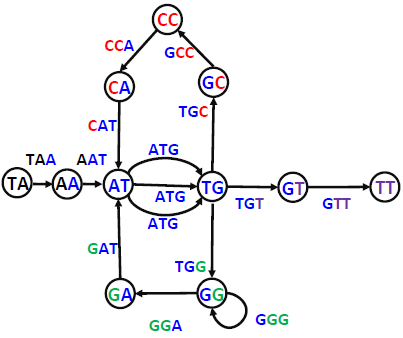
\includegraphics[width=0.6\textwidth]{poglavlja/3/slike/debrojnov.png}
	\caption{De Brojnov graf koji odgovara niski $TAATGCCATGGGATGTT$.}
	\label{slika:debrojnov}
\end{figure} 

Dobro, došli smo do nove reprezentacije niske pomoću grafa. Gde se sad nalazi naš \textit{Genome}? Kako nam se 3-grami sada nalaze na granama, a ne u čvorovima, potrebno je da pronađemo putanju u grafu koja prolazi sve grane tačno jednom. Takav put nazivamo \textit{Ojlerova putanja}. Srećom, algoritam za pronalaženje Ojlerove putanje u grafu nije NP-kompletan i možemo efikasno da je pronađemo.


\begin{problem}[Problem Ojlerove putanje]
	~\\ Pronaći Ojlerovu putanju u grafu.
	\\ Ulaz. Graf.
	\\ Izlaz. Putanja koja posećuje svaku granu u grafu tačno jednom.
\end{problem}


Sada znamo kako možemo da dobijemo nisku kada znamo de Brojnov graf koji odgovara njenom k-gramskom sastavu. Međutim, konstruisali smo de Brojnov graf na osnovu genoma, ali u realnim primenama, genom je nepoznat.


\section{De Brojnovi grafovi na osnovu kolekcije k-grama}

U redu, nije nam poznata niska, ali znamo njen k-gramski sastav. Za svaki k-gram pravimo dva čvora i jednu granu, na prethodno opisani način (\ref{slika:kgrami}).
Zatim lepimo identične čvorove sve dok ne dobijemo graf čiji svi čvorovi imaju različite oznake. Na slici je dat jedan korak ovog postupka, međutim tu nije kraj jer i dalje postoje čvorovi sa istim oznakama.

\begin{figure}[h]
	\centering
	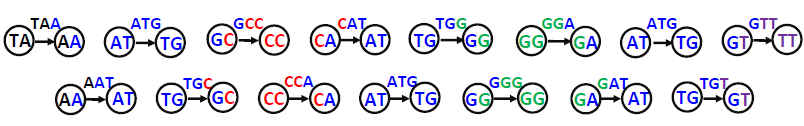
\includegraphics[width=1\textwidth]{poglavlja/3/slike/debrojnov1.png}
	\caption{Svaki k-gram prestavljen je pomoću dva čvora i jedne grane.}
	\label{slika:kgrami}
\end{figure} 

\begin{figure}[h]
	\centering
	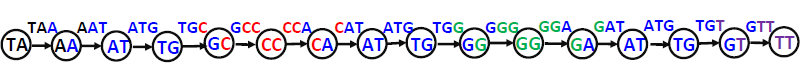
\includegraphics[width=1\textwidth]{poglavlja/3/slike/lepljenje.png}
	\caption{Postupak lepljenja čvorova. Posao nije završen!}
	\label{slika:lepljenje}
\end{figure} 


Po završetku postupka dobijamo de Brojnov graf koji je isti kao onaj koji smo dobili kada smo znali nisku. Svaka grana je označena jednim k-gramom. Svaki čvor je označen prefiksom/sufiksom izlazne/ulazne grane. Zalepljeni su svi čvorovi sa identičnim oznakama.

\section{Ojlerova teorema}

\begin{problem}[Problem Ojlerovog ciklusa]
	~\\ Pronaći ciklus Ojlerovom grafu.
	\\ Ulaz. Graf.
	\\ Izlaz. Ciklus koja posećuje svaku granu tačno jednom.
\end{problem}

\begin{teorema}[Ojlerova teorema]
	Svaki povezan graf i balansiran graf je Ojlerov.
\end{teorema}

Kažemo da je graf povezan ako za ma koja dva čvora postoji putanja koja ih povezuje.


%% MRAVI DOKAZUJU OJLEROVU TEOREMU

\begin{verbatim}
EulerianCycle(BalancedGraph)
form a Cycle by randomly walking in BalancedGraph (avoiding already visited edges)
while Cycle is not Eulerian
select a node newStart in Cycle with still unexplored outgoing edges
form a Cycle' by traversing Cycle from newStart and randomly walking afterwards
Cycle \leftarrow Cycle'
return Cycle
\end{verbatim}

\section{Sastavljanje parova očitavanja}

Od očitavanja do de Brojnovog grafa do genoma može se javiti više Ojlerovih putanja u grafu.

\subsection{DNK sekvenciranje sa parovima očitavanja} 

Imamo više identičnih kopija genoma i na slučajnim pozicijama sečemo genom na fragmente iste dužine \textit{InsertLength}. Zatim generišemo parove očitavanja: dva očitavanja sa krajeva svakog fragmenta na fiksiranoj udaljenosti.
Pod uparenim k-gramom podrazumevamo par k-grama na fiksiranom rastojanju d u genomu. Na primer, TCA i TCC na rastojanju d=11 čine jedan upareni k-gram.

\begin{problem} [Problem rekonstrukcije niske na osnovu parova očitavanja]
	~\\ Rekontruisati nisku na osnovu njenih uparenih k-grama.
	\\ Ulaz. Kolekcija uparenih k-grama.
	\\ Izlaz. Niska Text takva da je PairedComposition(Text) jednak kolekciji uparenih k-grama. 
\end{problem}

Kako konstruisati upareni de Brojnov graf na osnovu uparenog k-gramskog sastava?
Pretpostavimo da je dat genom (niska Genome). Posmatrajmo genom kao putanju u grafu obeleženom na osnovu njegovog uparenog kgramskog sastava.
\\
Pretpostavili smo da je dat genom (niska Genome). Posmatrali smo genom kao putanju u grafu obeleženom na osnovu njegovog uparenog k-gramskog sastava
\\
Sada pretpostavimo da nije dat genom već samo upareni k-gramski sastav

%% animacije, SVUDA ANIMACIJE!!!!!

~\\ Upareni de Brojnov graf na osnovu kolekcije uparenih k-grama:
\\ – Svaka grana je označena jednim uparenim k-gramom
\\ – Svaki čvor je označen prefiksima/sufiksima izlazne/ulazne grane
\\ – Zalepljeni su svi čvorovi sa identičnim oznakama.

\section{U realnosti}

Ovde smo imali neke nerealne pretpostavke.
\begin{itemize}
	\item  Savršena pokrivenost genoma očitavanjima (svaki k-gram iz genoma je očitan)
	\item Očitavanja ne sadrže greške
	\item Rastojanja između očitavanja u okviru parova očitavanja su egzaktna
	\item Nesavršena pokrivenost genoma očitavanjima (svaki k-gram iz genoma je očitan)
	\\ Očitavanja ne sadrže greške
	\\ Rastojanja između očitavanja u okviru parova očitavanja nisu egzaktna
\end{itemize}

\subsection{Savršena pokrivenost}

Prva nerealna pretpostavka je savršena pokrivenost.
\\
Očitavanja dužine 250 nukleotida dobijena Illumina tehnologijom predstavljaju samo mali deo 250-grama unutar genoma.
\\
Rešenje: razbiti dobijena očitavanja na kraće k-grame
\\
\\
Druga nerealna pretpostavka: očitavanja ne sadrže greške.

\newpage
\section{Zadaci sa vežbi}
U nastavku će biti predstavljeni zadaci sa vežbi na kursu rađeni u programskom jeziku Python.





\backmatter
\renewcommand{\bibname}{Literatura}

\begingroup
\raggedright
\bibliography{bioinformatika}
\endgroup

\bibliographystyle{ieeetr}
\addcontentsline{toc}{chapter}{Literatura}

\end{document}